\section{외관 검사}
외관 검사의 목적은 포일의 형태를 검사하는 것으로 그림 \ref{fig:light_board}와 같이 메카로 품질검증실에 마련된 필름판독기에 포일을 올리고 진행한다.

\begin{figure}[htb]
  \centering
  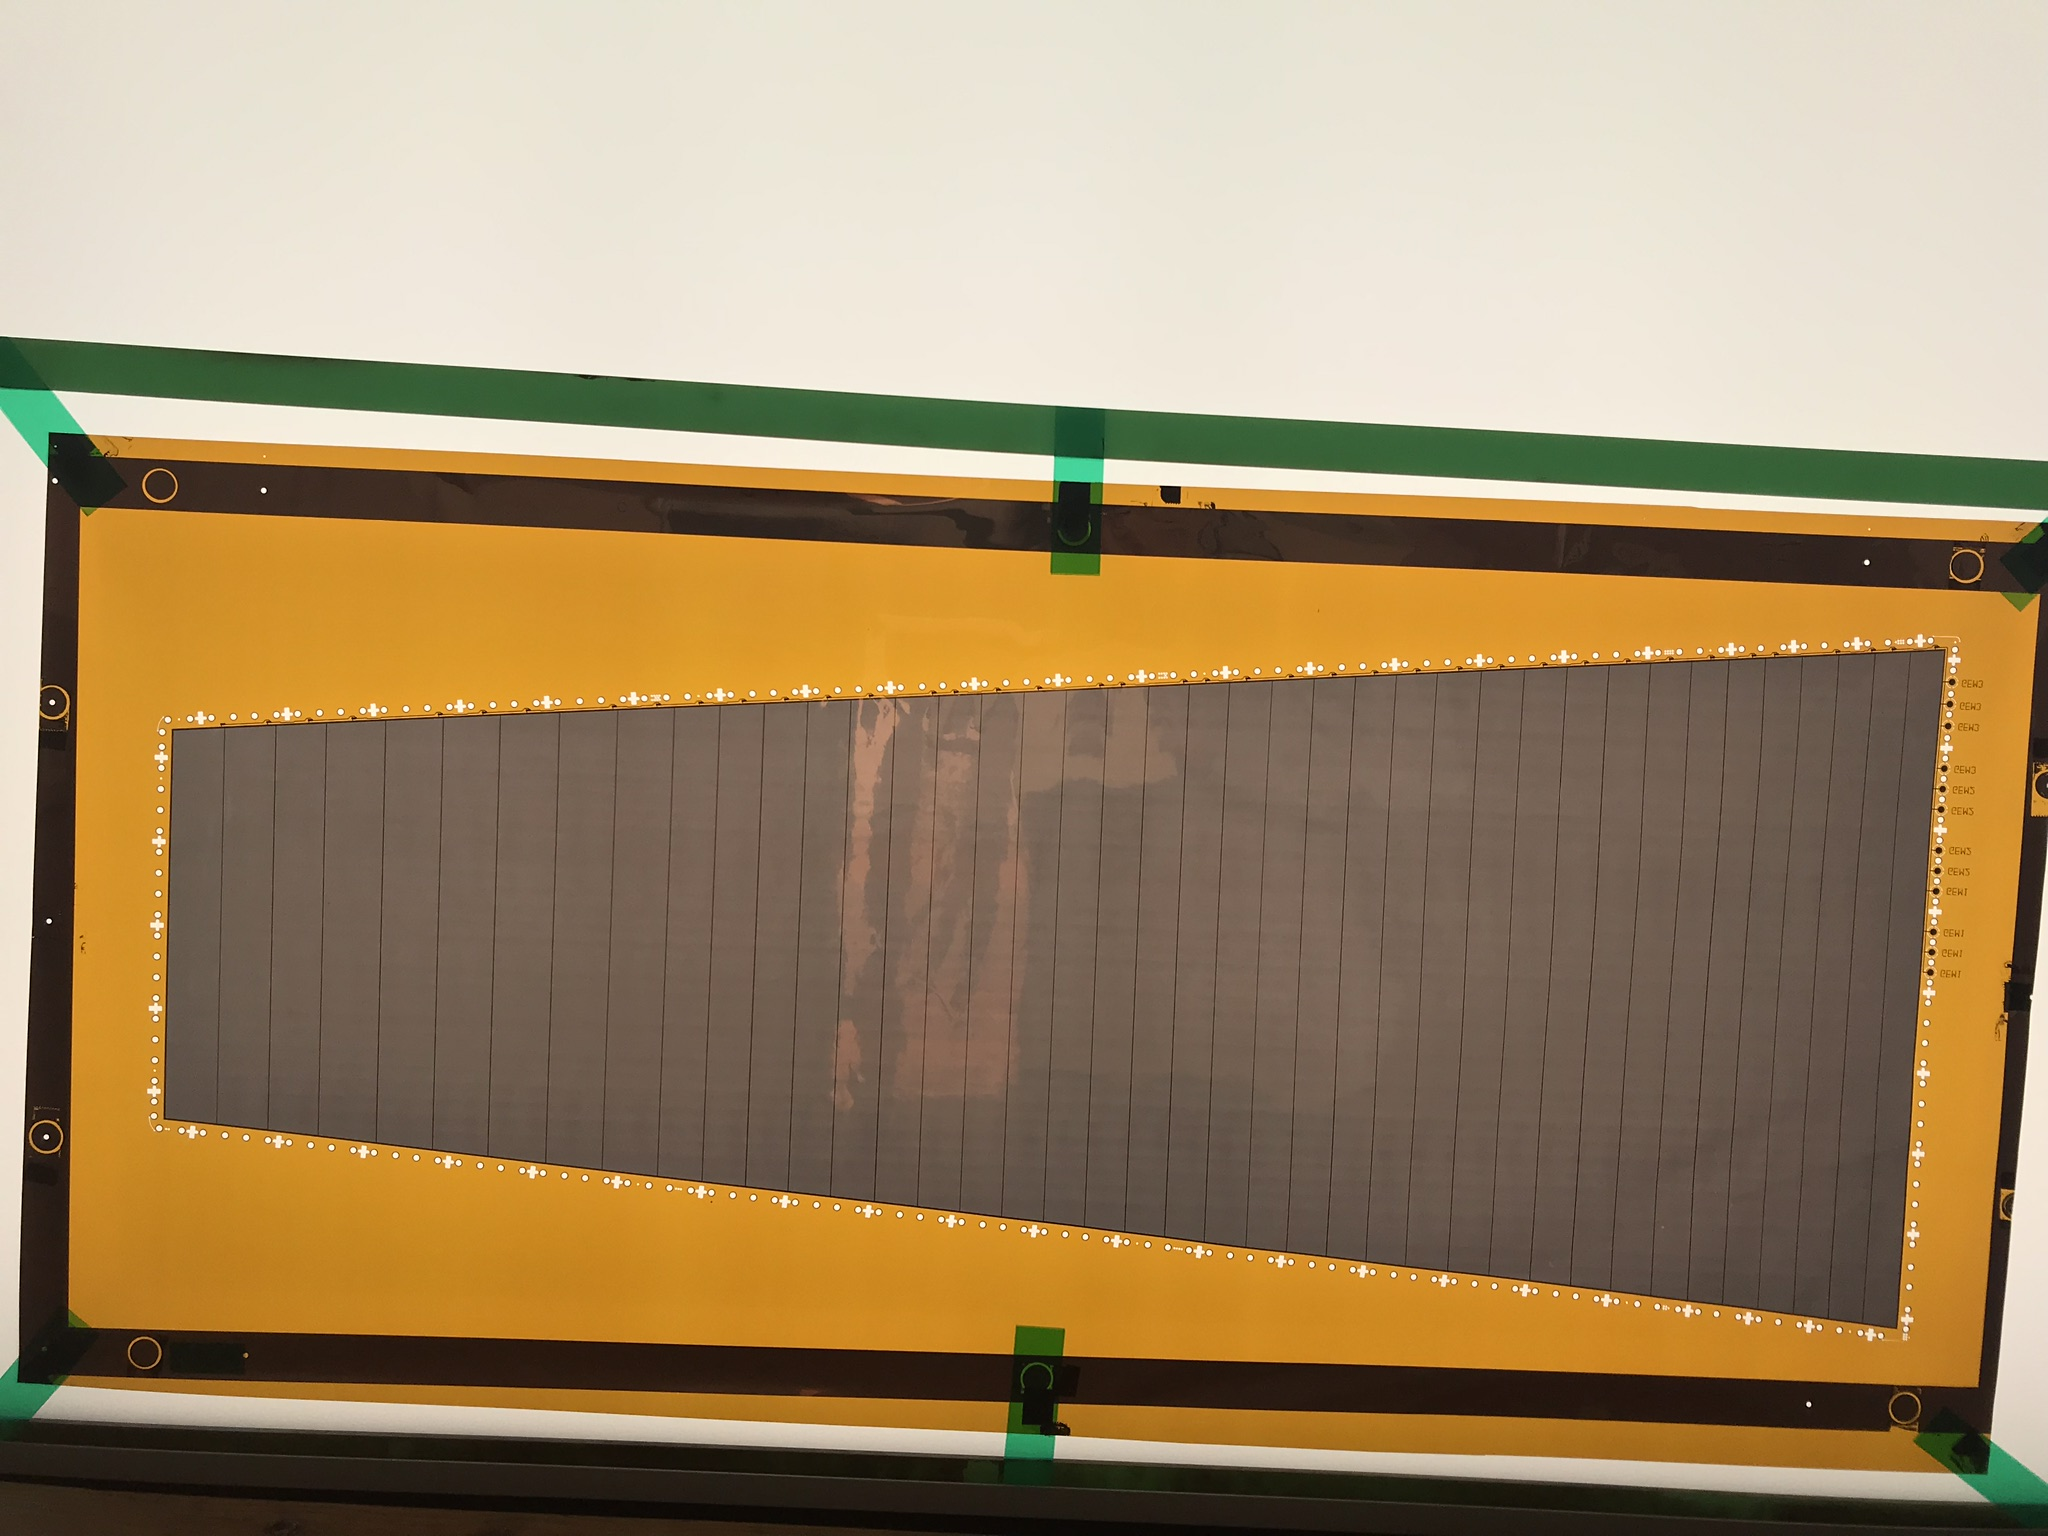
\includegraphics[width=0.60\textwidth]{Light_Board.jpg}
  \caption[대형 GEM 포일을 필름 판독기에 놓은 모습]{대형 GEM 포일을 필름 판독기에 놓은 모습. 결함이 있는 부분은 다른 곳보다 밝게 보이므로, 결함을 쉽게 확인할 수 있다.}
  \label{fig:light_board}
\end{figure}

외관 검사에서 실패한 포일은 포일의 상태에 따라 \uline{인수거부 또는 추가 공정을 의뢰}해야 한다. 자세한 행동 요령은 각 항목을 참조할 것.

\uline{외관 검사를 진행해야 되는 포일들을 청결 검사를 진행하는 포일들과 섞이지 않도록 공간상으로 분리할 것.} 

\subsection{은 페이스트 건조 검사}
가장 먼저 HV 패드에 은 페이스트가 완전히 건조 되었는지 검사한다. 건조되지 않은 은 페이스트가 포일을 취급하는 중에 밀려 GEM 포일의 활성 영역에 들어가면, 포일이 달락되며 이를 복구할 수 없다. 따라서 은 페이스트의 건조 여부를 가장 먼저 확인한다. 그림 \ref{fig:undried_paste}은 은 페이스트가 완전히 건조되지 않은 상태에서 포장을 진행하였기 때문에 발생한 현상이다. 은 페이스트가 주변으로 밀려들어간 것을 확인할 수 있다.

\uline{만약 HV 패드에 은 페이스트가 발라져 있지 않을 경우, 메카로 직원에게 이를 알리고 페이스트 도포를 의뢰한다.}

\begin{figure}[htb]
  \centering
  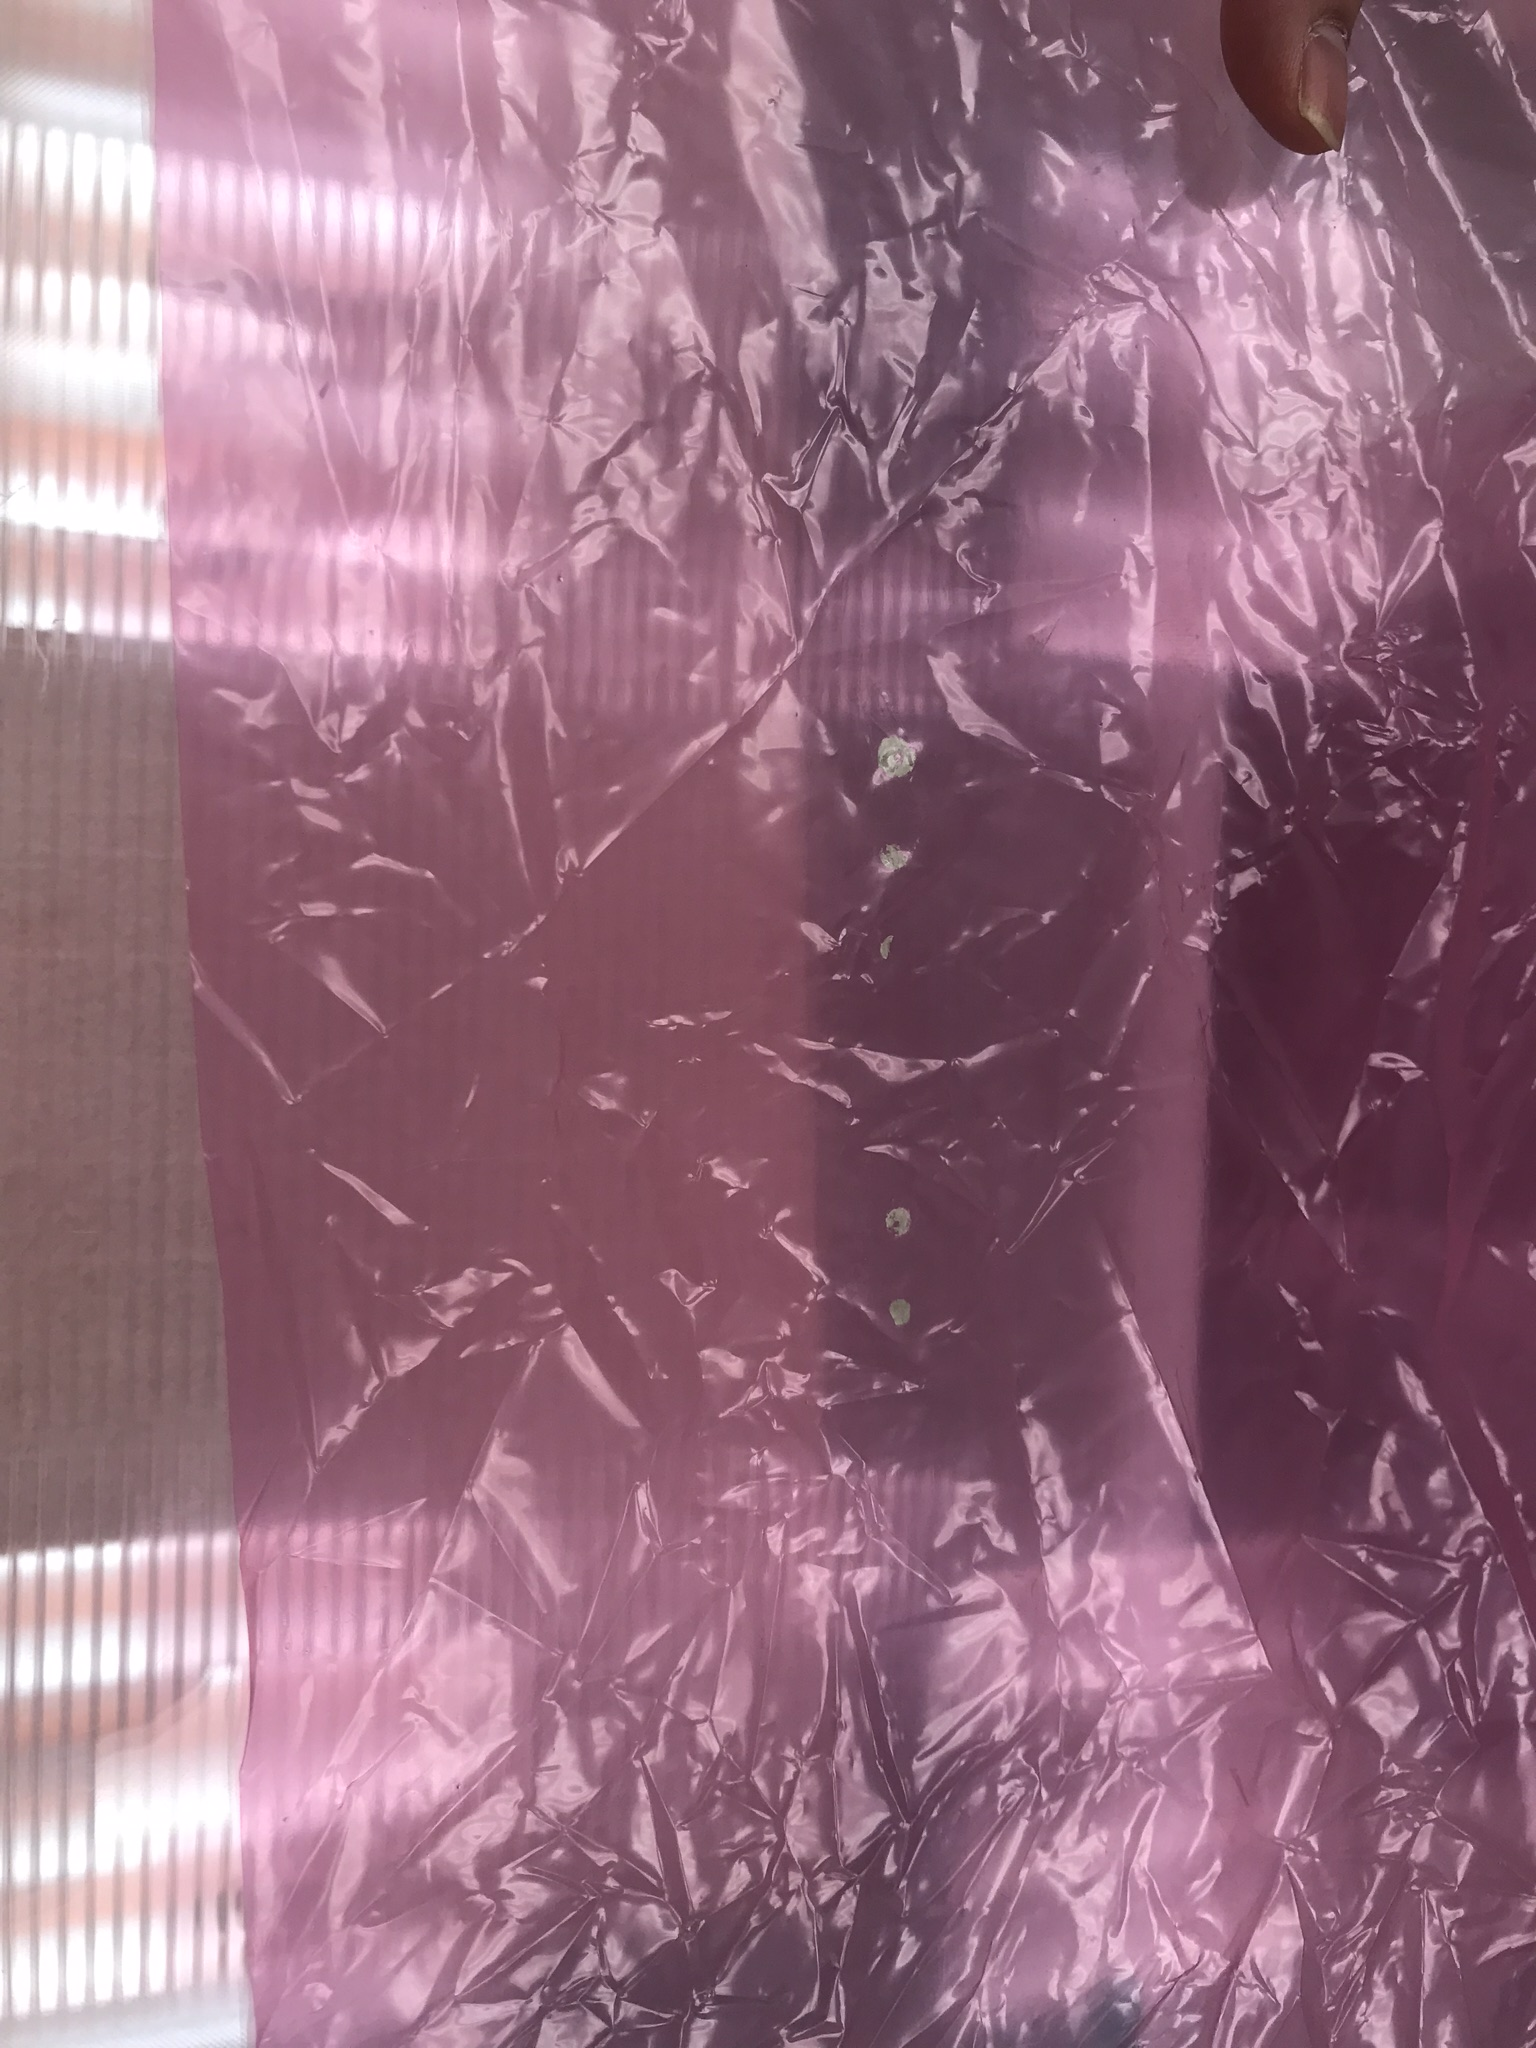
\includegraphics[width=0.40\textwidth]{Undried_Silver_Paste.jpg}
  \caption[건조되지 않은 은 페이스트]{은 페이스트가 완전히 건조되지 않은 상태에서 포장을 진행했을 때, 발생하는 현상. 방정전 필름에 은 페이스트가 묻은 것을 확인 할 수 있다. 이 때 은 페이스가 주변으로 밀려 들어가게 된다.}
  \label{fig:undried_paste}
\end{figure}

\subsection{홀 지름 검사}
GEM 홀의 지름이 목표치인 PI홀 (구리홀) \SI{50}{\micro\meter} (\SI{70}{\micro\meter})에 도달했는지 검사한다.

GE2/1 M7 1차 배송분에서, PI홀의 지름이 목표치보다 작은 포일이 발견되었다. 이는 식각 용액의 휘발에 따라 식각 특성이 많이 변하기 때문이며, 메카로의 시각 용액의 품질 표준화가 충분하게 진행되지 않기 때문이다. PI홀의 지름은 GEM 검출기의 이득에 영향을 주기 때문에 PI홀의 지름을 일정하게 유지하는 것이 중요하다. 또한 PI홀의 지름이 일정하게 나오지 않는다는 것은 PI 에칭 조건이 틀렸음을 암시하기 때문에 홀의 전반적인 구조가 틀렸을 가능성을 암시한다. 그리고 PI 에칭 조건이 틀렸을 경우, 식각 결합의 치명성을 유도하기도 한다. 따라서 PI홀의 지름은 $\SI{50}{\micro\meter}\pm\SI{3}{\micro\meter}$ 수준을 유지해야 한다.

구리홀의 경우 그간 큰 문제 없이 $\SI{70}{\micro\meter}\pm\SI{2}{\micro\meter}$을 유지하였다. 메카로의 공정 방식을 생각하였을 때, 앞으로도 구리홀의 지름 표준화에는 문제가 없을 것으로 예상한다.

PI홀 (구리홀)의 지름은 필름 판독기에 설치되어 있는 현미경과 컴퓨터 SW을 이용하여 측정한다. PI홀과 구리홀의 구분은 빛을 포일의 아래에서 쏘여 주거나 위에서 쏘여 주는 방식으로 할 수 있다. 빛을 포일의 아래에서 쏘여 주면 PI홀의 지름을 측정할 수 있고, 빛을 포일의 위에서 쏘여 주면 구리홀의 지름을 측정할 수 있다. 현미경의 초점을 정확하게 맞춘 후 측정을 진행해야 한다.

홀 지름은 포일의 네 모퉁이와 가운데 다섯 곳에서 측정한다. 홀 지름 검사는 PI 식각일 기준으로 하루 생산분에서 하나의 포일에만 진행하면 된다. \uline{만약 하나의 포일에 문제가 발견되었을 경우, PI 식각일 기준으로 같은 날에 생산된 다른 포일에도 문제가 있을 가능성이 매우 높다.} 따라서 이 경우에는 해당 포일들에 대한 검사를 철저히 진행해야 한다.
 
\uline{홀 지름에 문제가 있는 포일은 인수 거부되어야 한다.}

\subsection{식각 결함 검사}
공정의 특성상 그림 \ref{fig:example_defect}와 같은 식각 결함이 발생할 수 있으며 일정 부분 불가피한 면도 있는다. 하지만 식각 결함을 점차 줄이는 것이 바람직하다. 따라서 KCMS 구성원들은 공정의 보완을 위해 식각 결합의 빈도를 추적해야 한다. 그리고 치명적 형태의 식각 결함이 있는 포일을 걸러내야 한다. 

그림 \ref{fig:example_defect}의 왼쪽 사진처럼 구리층만 손상되었고 PI층이 온전한 경우, 대체로 큰 문제는 없다. 단지 해당하는 활성 영역을 잃을 뿐이고, 검출기를 운영하는데 그외의 문제가 발생하지 않기 때문이다. 정해진 기준은 없으나, 결함 면적이 \SI{5}{\milli\meter\squared} 이하라면 충분히 감수가능하다고 생각된다. 다만 이런 양상의 결함은 드물다.

\begin{figure}[htb]
  \centering
  \subfloat[구리층이 손상된 포일]{
    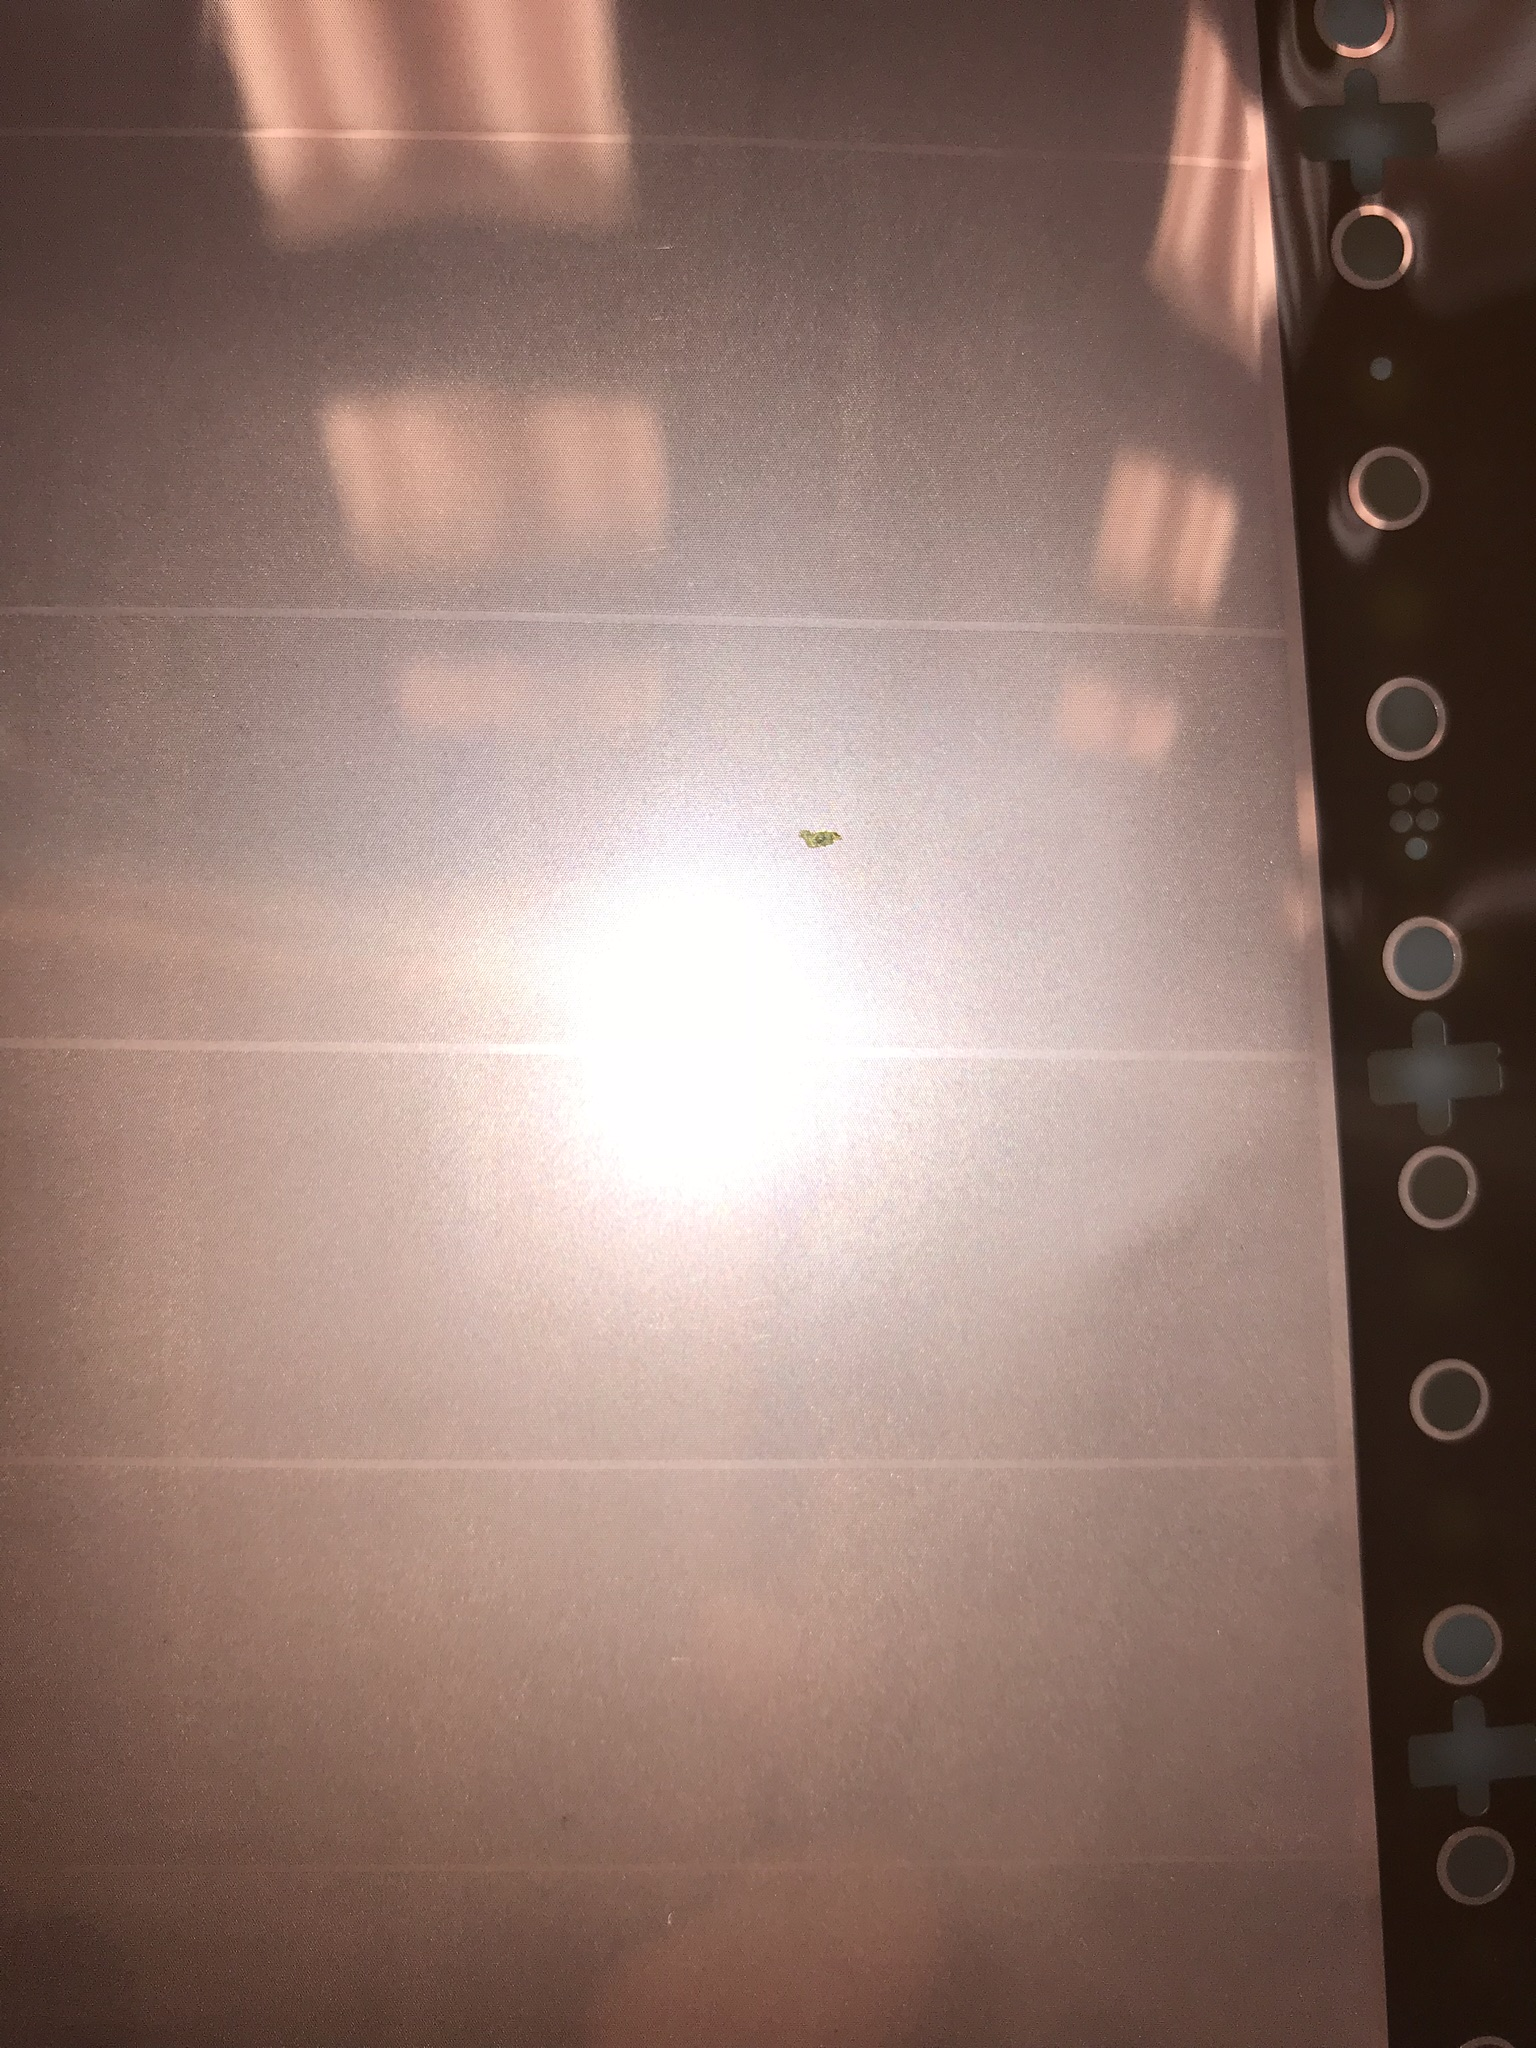
\includegraphics[width=0.40\textwidth]{Defect_OK.jpg}
  }
  \subfloat[PI층까지 손상된 포일]{
    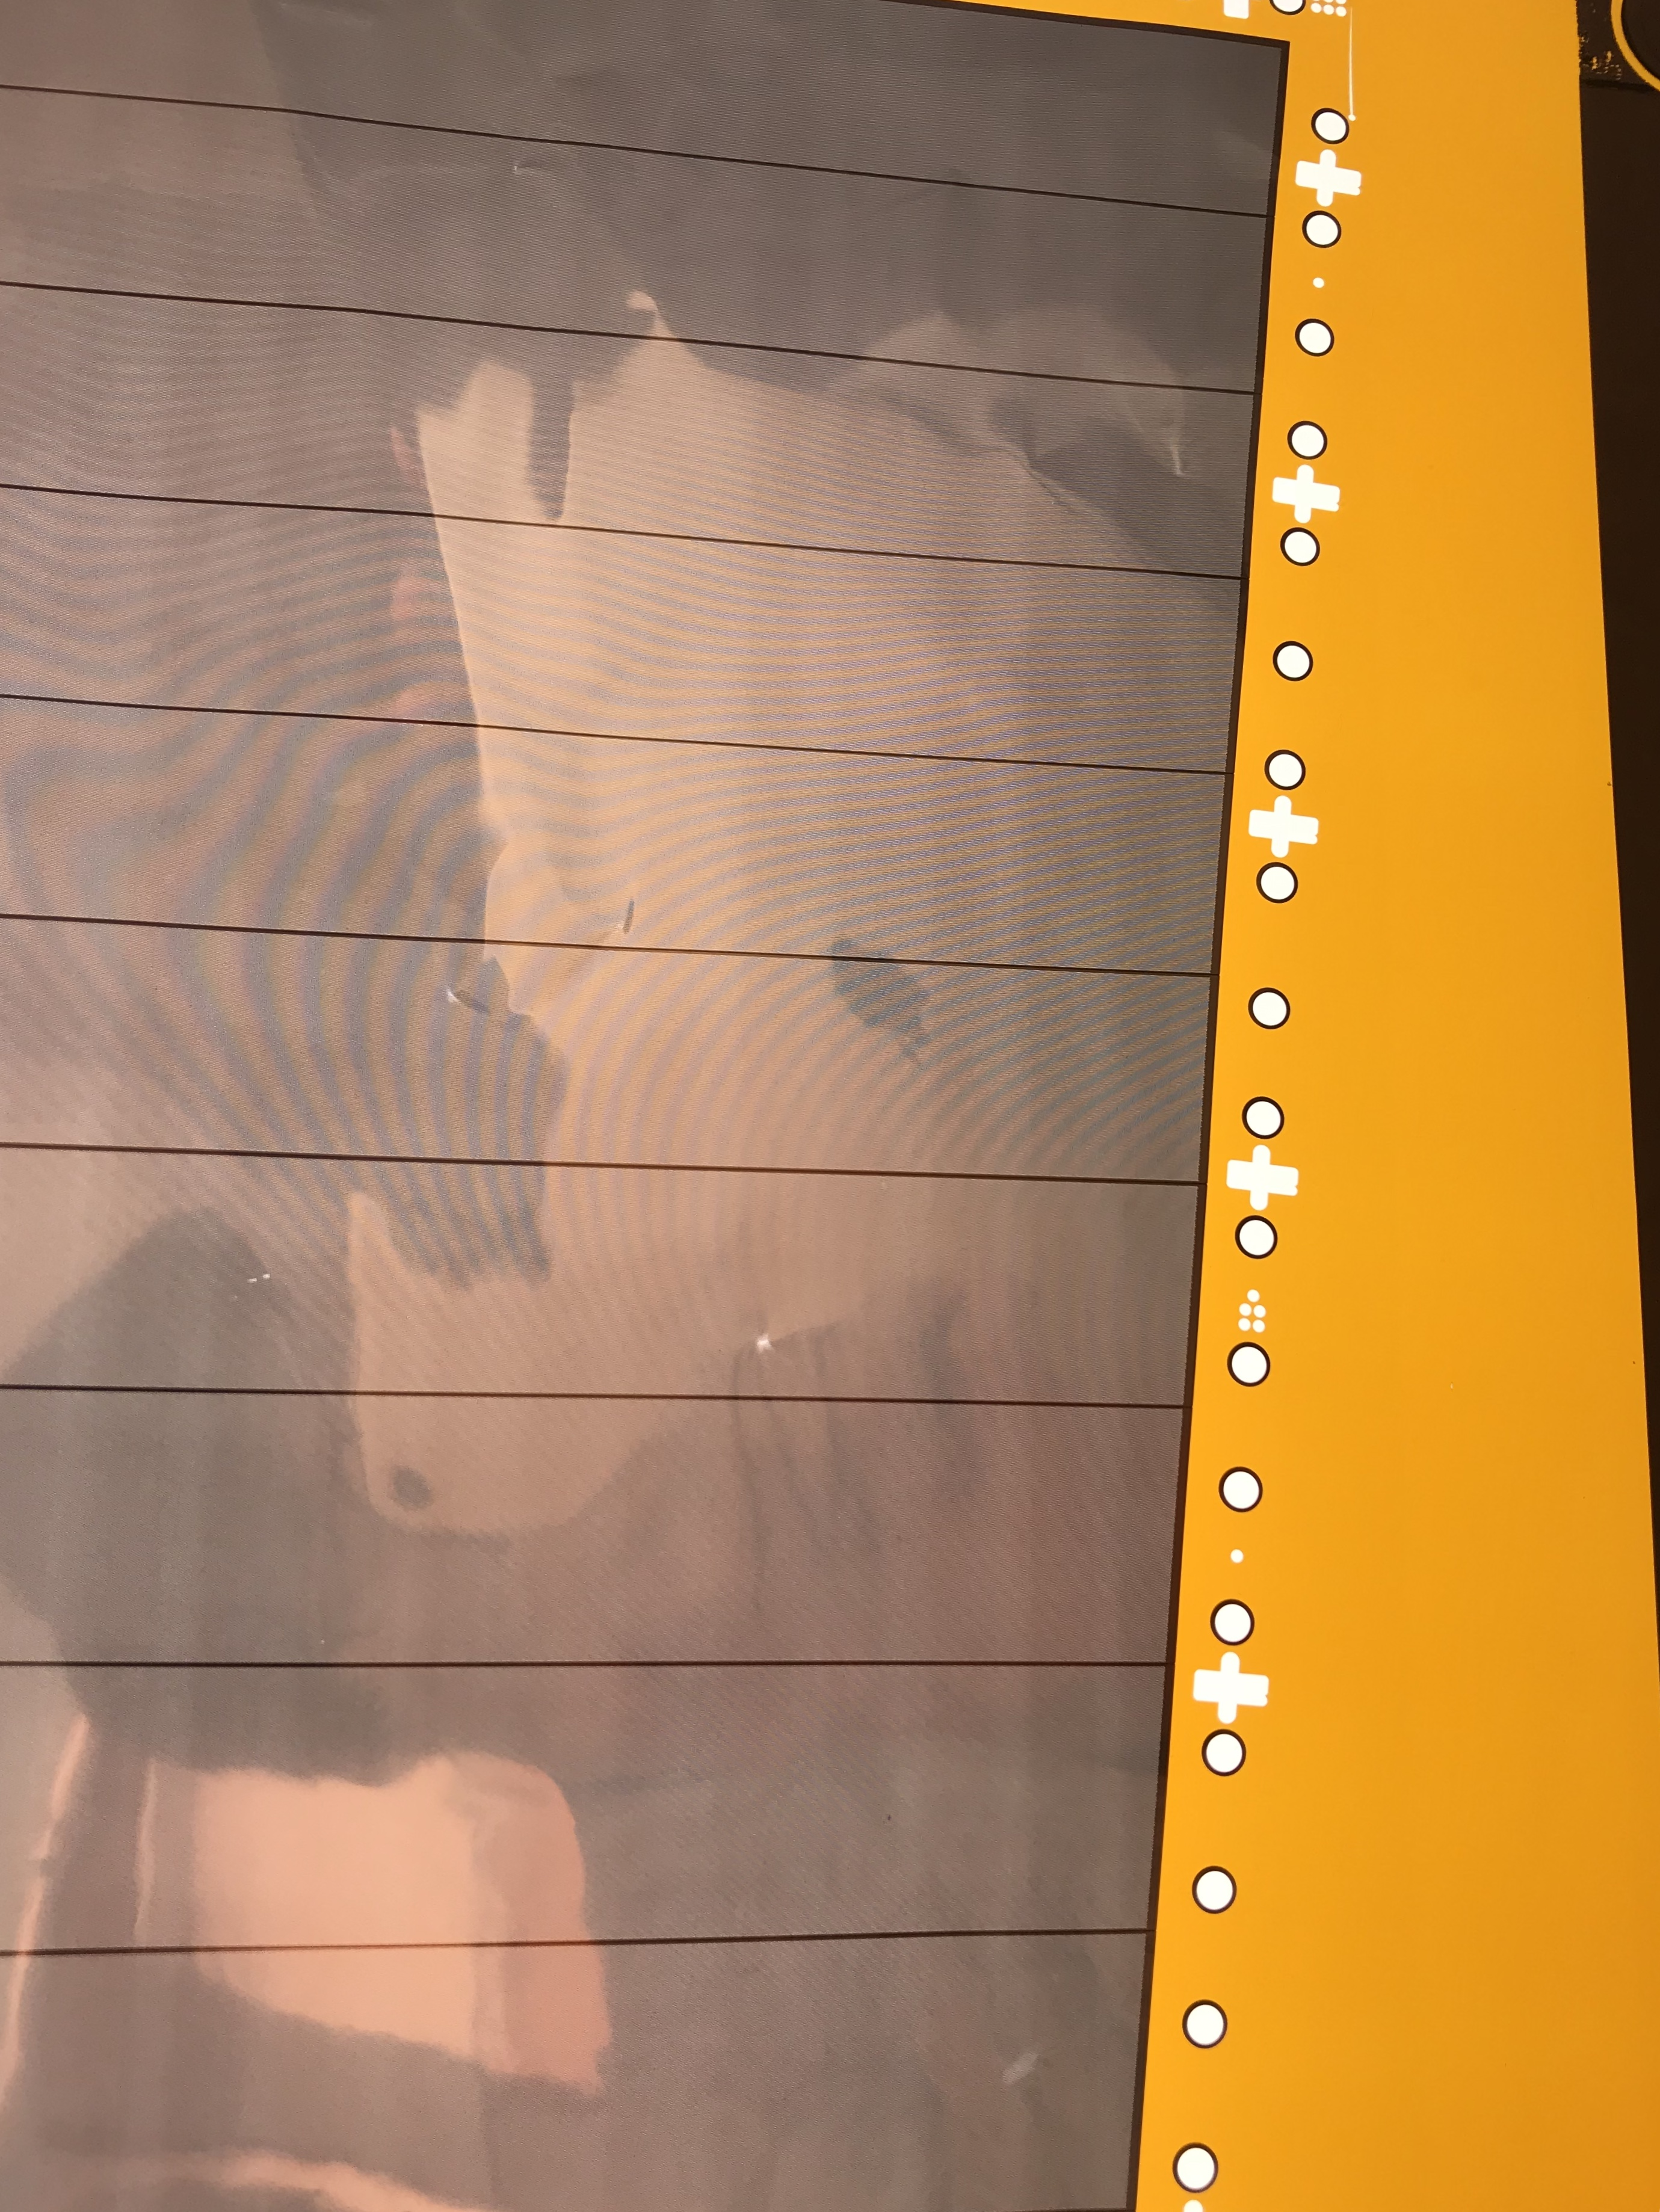
\includegraphics[width=0.40\textwidth]{Defect_Bad.jpg}
  }
  \caption[식각 결합의 예]{식각 결합의 예. (왼쪽) PI층이 온존한 경우이다. PI층이 온존하기 때문에 결함 위치가 진한 노란색으로 보인다. (오른쪽) 그림은 PI층이 파괴되었으며 부분적으로 온전한 구리층이 사라진 PI층 위를 살짝 덮고 있는 형태이다. PI층이 사라졌기 때문에 결함의 중심부가 하얀색으로 보인다.}
  \label{fig:example_defect}
  \end{figure}

대다수의 식각 결합의 경우 그림, \ref{fig:example_defect}의 오른쪽 사진처럼 PI층까지 손상을 입는다. PI층이 사라졌기 때문에 결함의 중심부가 하얀색으로 보인다. 이 경우 남아 있는 구리층의 형태에 따라 매우 중대한 결함이 될 수도 있고 아닐 수도 있다. \uline{위험성은 남아있는 구리층이 접촉되어 단락을 일으킬 가능성을 예측하여 판단한다.} 필요한 경우 현미경을 통해 손상 양상을 확인한다.  만약 PI층의 파괴 범위보다 구리층의 파괴 범위가 더 넓어서 두 구리층이 접촉 가능성이 없는 형태라면, 결함 면적에 따라 큰 문제가 없을 수 있다. 만약 남아 있는 구리층에 뾰족한 부분이 있다면 구리층이 단락될 가능성이 높을 것이다. 또한 PI층 없이 남아 있는 구리층이 넓으면 구리층이 단락될 가능성이 높을 것이다. 상당 부분 작업자의 경험과 감에 의존할 수 밖에 없는 부분이다.

그림 \ref{fig:defect_bad_zoom}은 이와 같은 치명적 결합의 양상을 보여준다. 하얀색으로 보이는 부분은 구리층과  PI층이 모두 파괴된 영역이고, 연한 갈색으로 보이는 부분은 PI층 없이 구리층만 남아 있는 영역이다. 구리층만 남아 있는 영역이 상당히 넓어서 포일이 단락될 가능성이 매우 높다.

만약 결함이 포일이 구겨진 위치에 존재한다면, 해당 포일은 특히 신중하게 검사를 진행해야 한다. 치명적 결함은 구겨진 FCCL에 식각 작업을 진행했을 때 발생할 수 있는 것으로 알려져 있다. 그림 \ref{fig:defect_bad_zoom}을 보면 사진상 흐릿하지만, 포일이 구겨진 것을 확인할 수 있다. 구김으로 생긴 모서리에 결함이 위치한 것을 확인할 수 있다. 따라서 \uline{구김 위에 있는 결함이 있을 경우 특히 신중하게 검사를 진행해야 한다.}

\uline{단락 가능성이 높아 보이는 치명적 결함이 발생했을 경우, 해당 포일은 인수 거부되어야 한다.}

\begin{figure}[htb]
  \centering
  \subfloat[치명적 결합의 육안 사진]{
    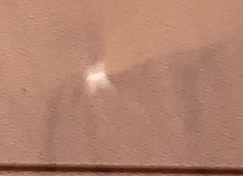
\includegraphics[width=0.40\textwidth]{Defect_Bad_Zoom.png}
  }
  \subfloat[치명적 결함의 현미경 사진]{
    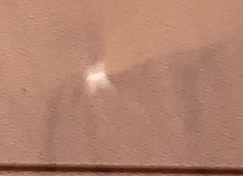
\includegraphics[width=0.40\textwidth]{Defect_Bad_Zoom.png}
  }
  \caption[치명적 식각 결함의 양상]{(왼쪽) 치명적 결함의 육안 사진이다. PI층이 파괴되었으며 부분적으로 온전한 구리층이 사라진 PI층 위를 살짝 덮고 있는 형태이다. PI층이 사라졌기 때문에 결함 위치가 하얀색으로 보이며, 부분적으로 온전한 구리층이 연한 갈색으로 보인다. (오른쪽) 칠명적 결함의  현미경 사진이다. (추후 업데이트 예정)}
  \label{fig:defect_bad_zoom}
    \end{figure}

\subsection{SMD 저항 검사}
SMD 저항이 빠짐 없이 그리고 정상적인 위치에 납땜이 되어 있는지 검사해야 한다. \uline{SMD 저항이 한두개 씩 납땜 되지 않는 경우가 굉장히 빈번}하므로 꼼꼼하게 검사해야 한다. SMD 저항이 잘못 납땜된 예시는 그림 \ref{fig:bad_solder}와 같다.

\uline{납땜이 되지 않은 섹션을 발견하면 메카로에 납땜과 이소프로필알콜 또는 아세톤으로 납땜 찌꺼기의 세척 후 포일 재세척을 의뢰한다.}

\begin{figure}[htb]
  \centering
  \subfloat[]{
    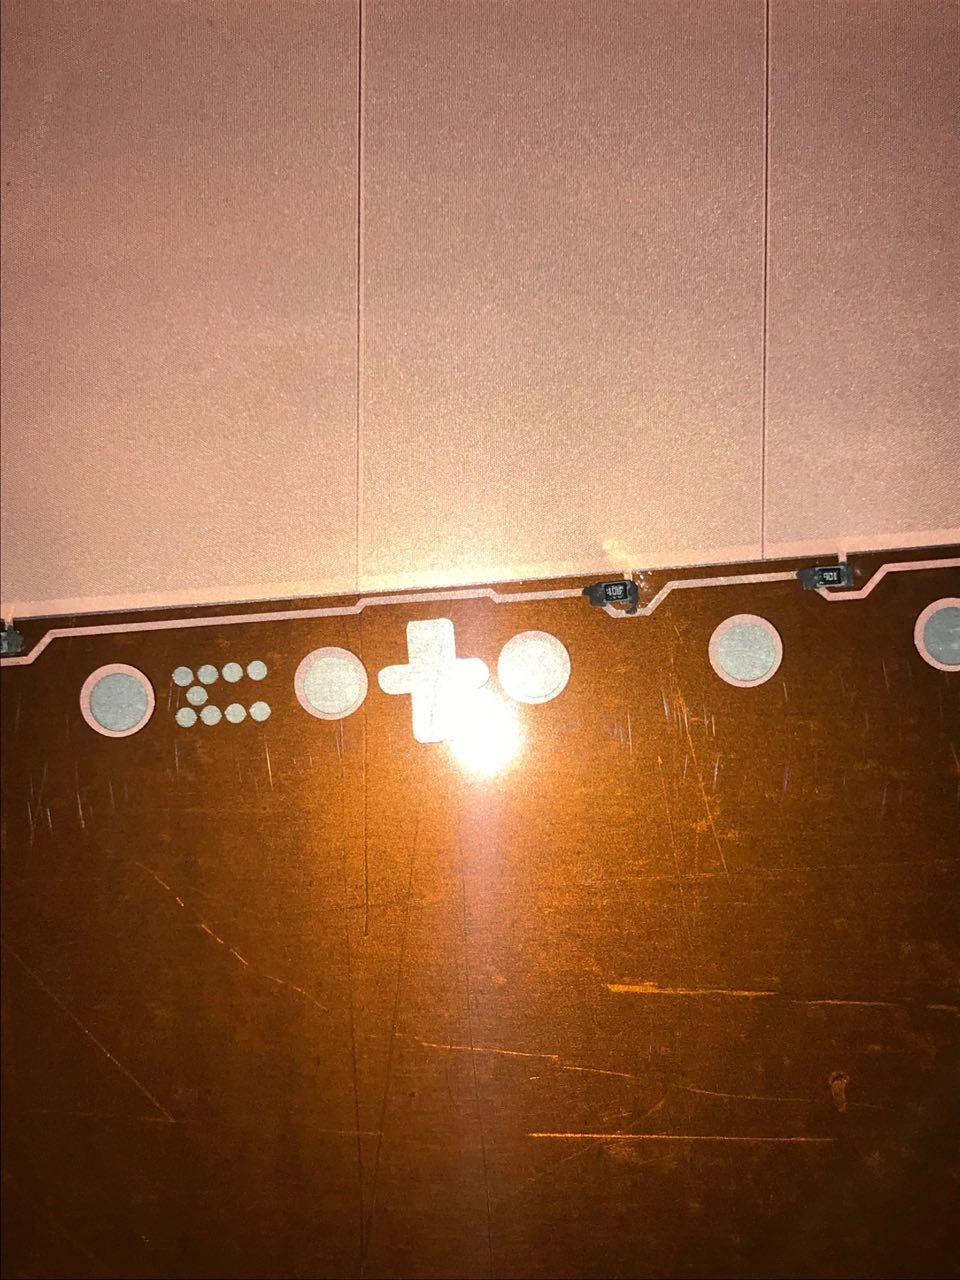
\includegraphics[width=0.30\textwidth]{bad_solder_0.jpg}
  }
  \subfloat[]{
    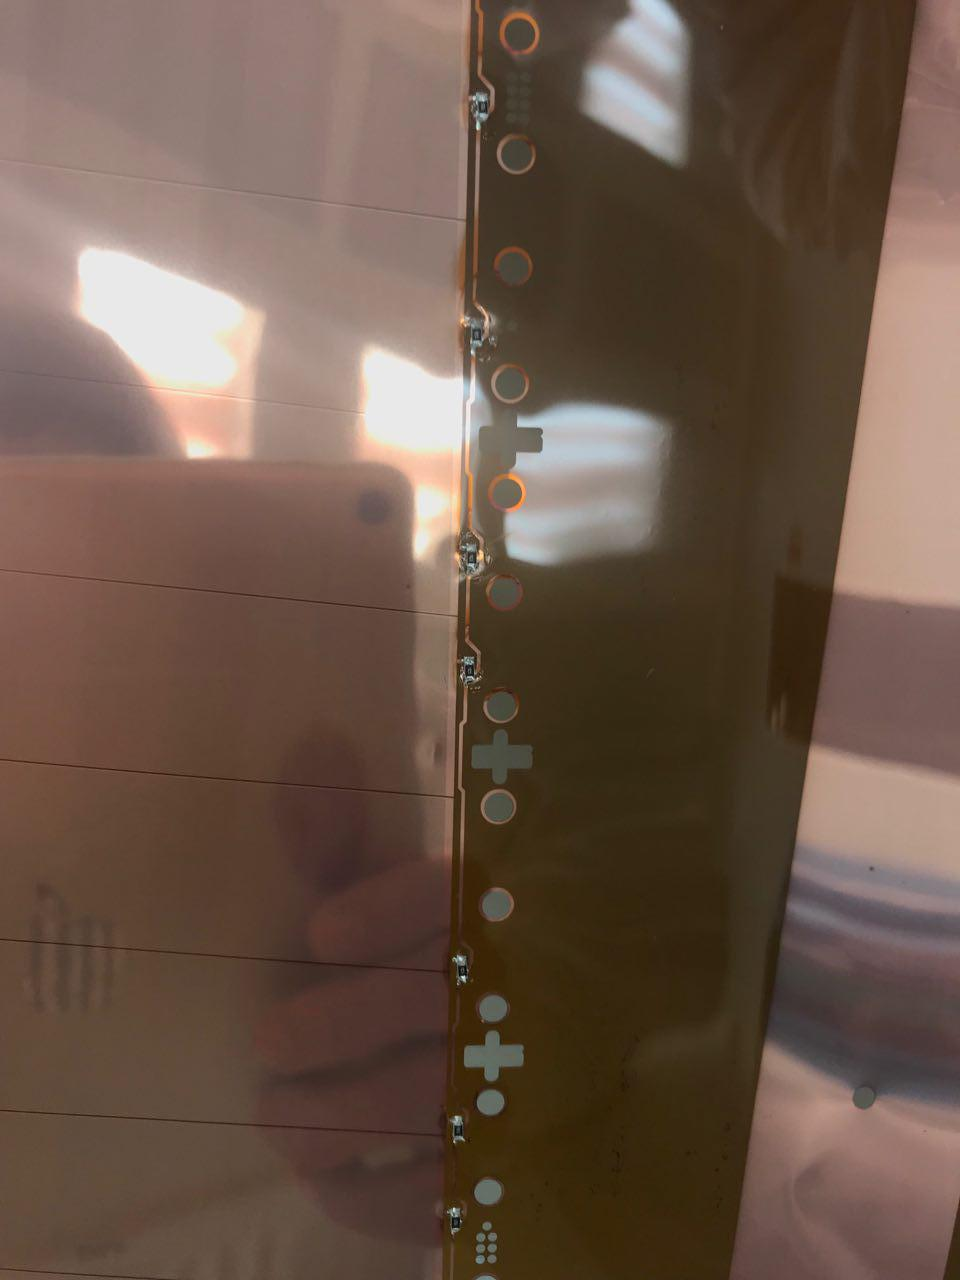
\includegraphics[width=0.30\textwidth]{bad_solder_1.jpg}
  }
  \subfloat[]{
    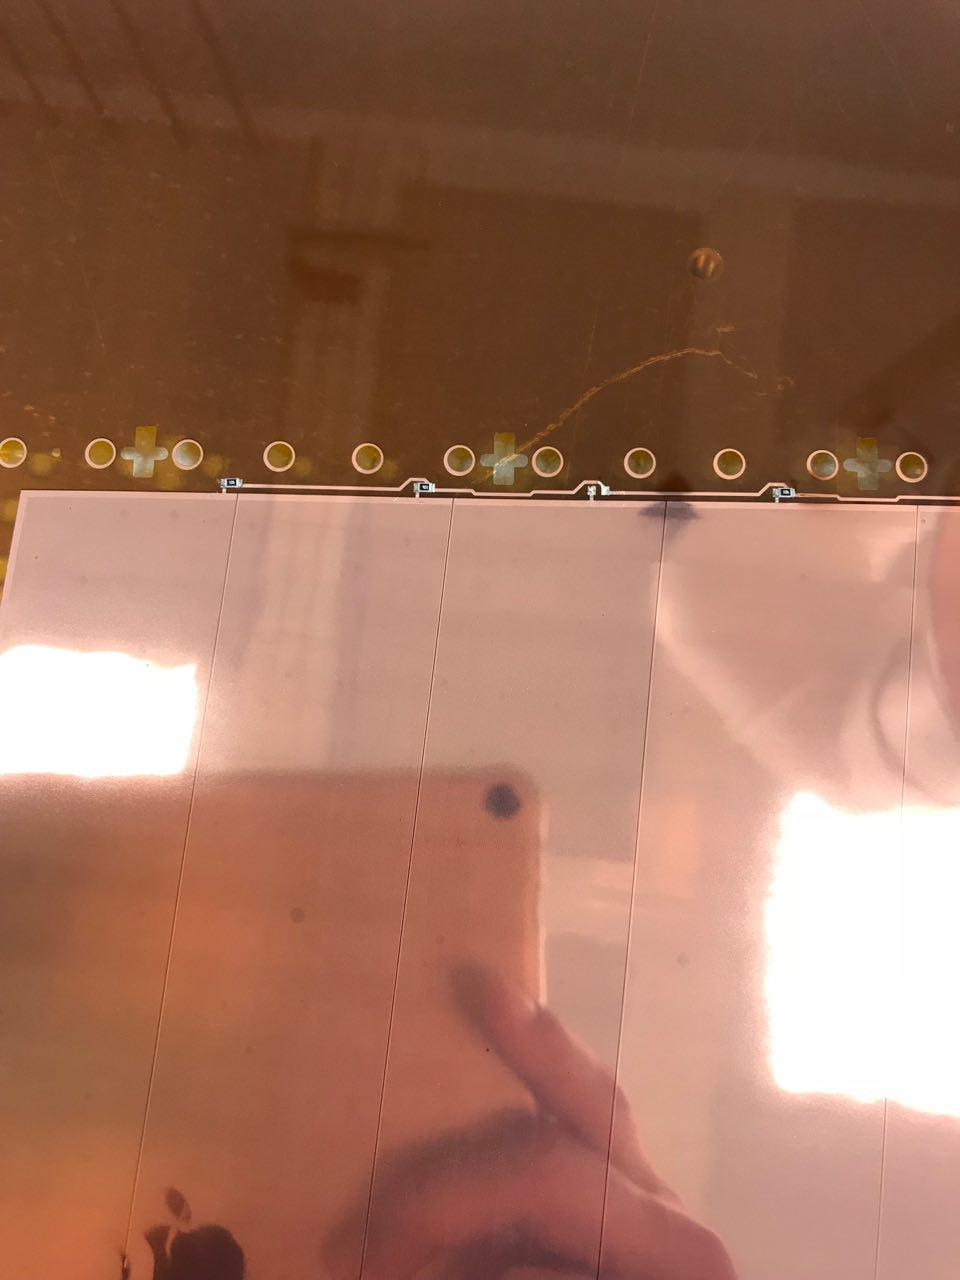
\includegraphics[width=0.30\textwidth]{bad_solder_2.jpg}
  }
  \caption[SMD 저항 납땜이 잘못된 예]{SMD 저항 납땜이 잘못된 예들. (왼쪽) 과도한 땜납이 다른 전극선을 침범함. (중간) 과도한 온도로 납땜을 하여 구리층이 산화됨. (오른쪽) SMD 저항이 납땜되지 않았음.}
  \label{fig:bad_solder}
\end{figure}

\subsection{전극선 단선 검사}
전극선에 끊어진 곳이 없이 정상적으로 형성이 되어 있는지 검사해야 한다. \uline{멀티미터로 전극선 양끝의 저항을 측정하여 단선이 있는지 확인한다.} 그림 \ref{fig:hv_line_cut}이 보여 주는 것처럼, 눈으로는 단선을 확인할 수 없는 경우가 대부분이다. 전극선 단선은 굉장히 빈번한 결합 양상이므로 꼼꼼하게 검사해야 한다. 전극선은 저항 주변에서 끊어지는 경우가 많다.

\uline{만약 단선이 있을 경우 위치를 찾아 메카로에 알리고, 은 페이스트로 수리할 것을 의뢰한다.}

\begin{figure}[htb]
  \centering
  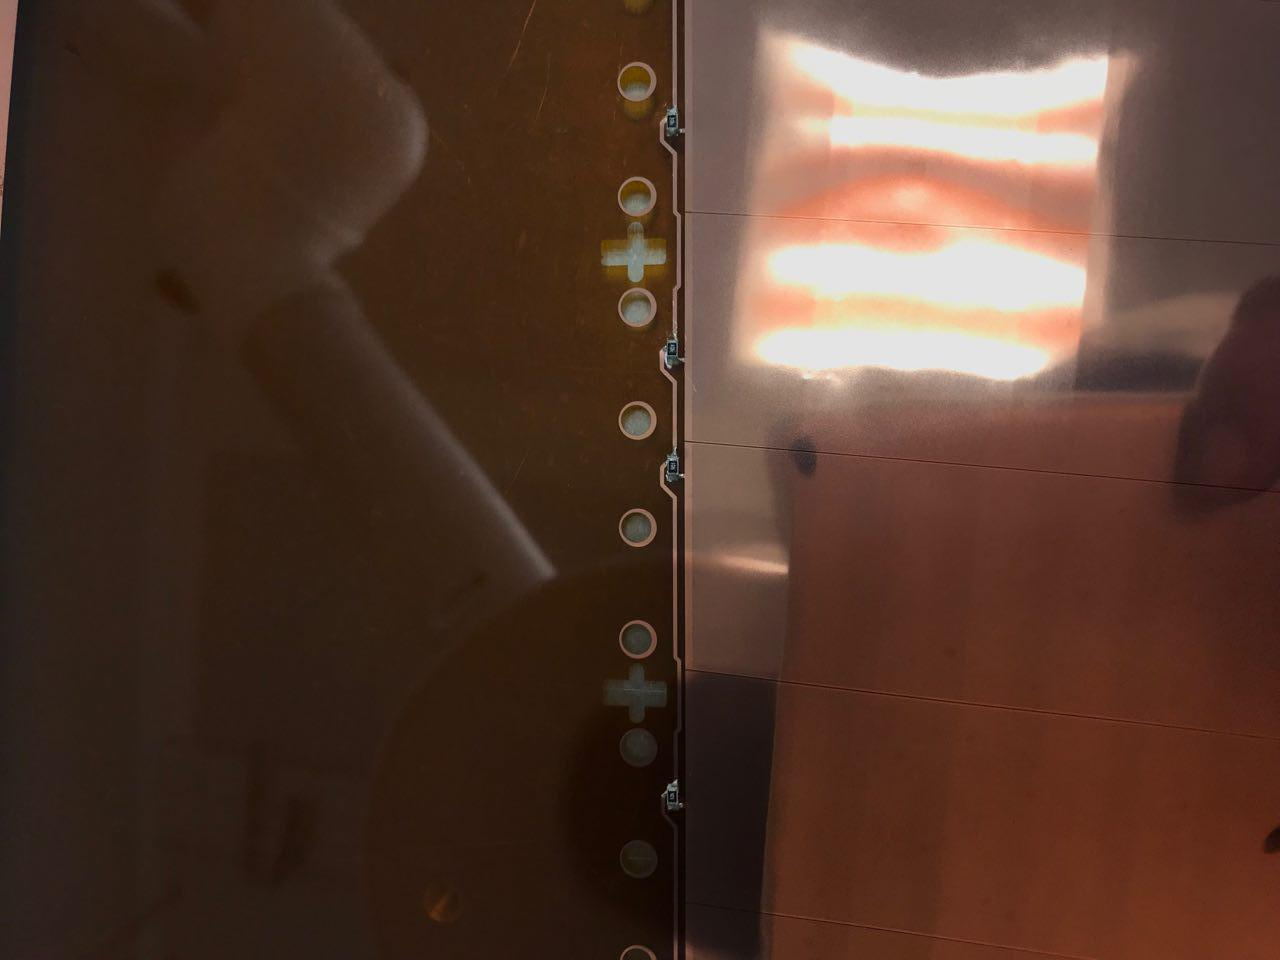
\includegraphics[width=0.50\textwidth]{hv_line_cut.jpg}
  \caption[전극선 단선의 예]{전극선 단선의 예. 위쪽에서 2번째 SMD 저항의 윗쪽 전극 주변의 전극선이 단선되었다.}
  \label{fig:hv_line_cut}
\end{figure}

\subsection{구겨짐 확인}
그림 \ref{fig:example_damaged_foils}처럼 공정 과정 상 어쩔 수 없이 발생하는 작은 구겨짐 외에 찍힘, 또는 접힘 등의 물리적 손상이 보일 경우, 포일의 장기간 안정성을 보장할 수 없다. 메카로의 경험이 쌓이면서 급격히 줄어 들고 있는 결합 양상이다.

\uline{구겨진 포일은 인수 거부되어야 한다.}

\begin{figure}[htb]
  \centering
  \subfloat[]{
    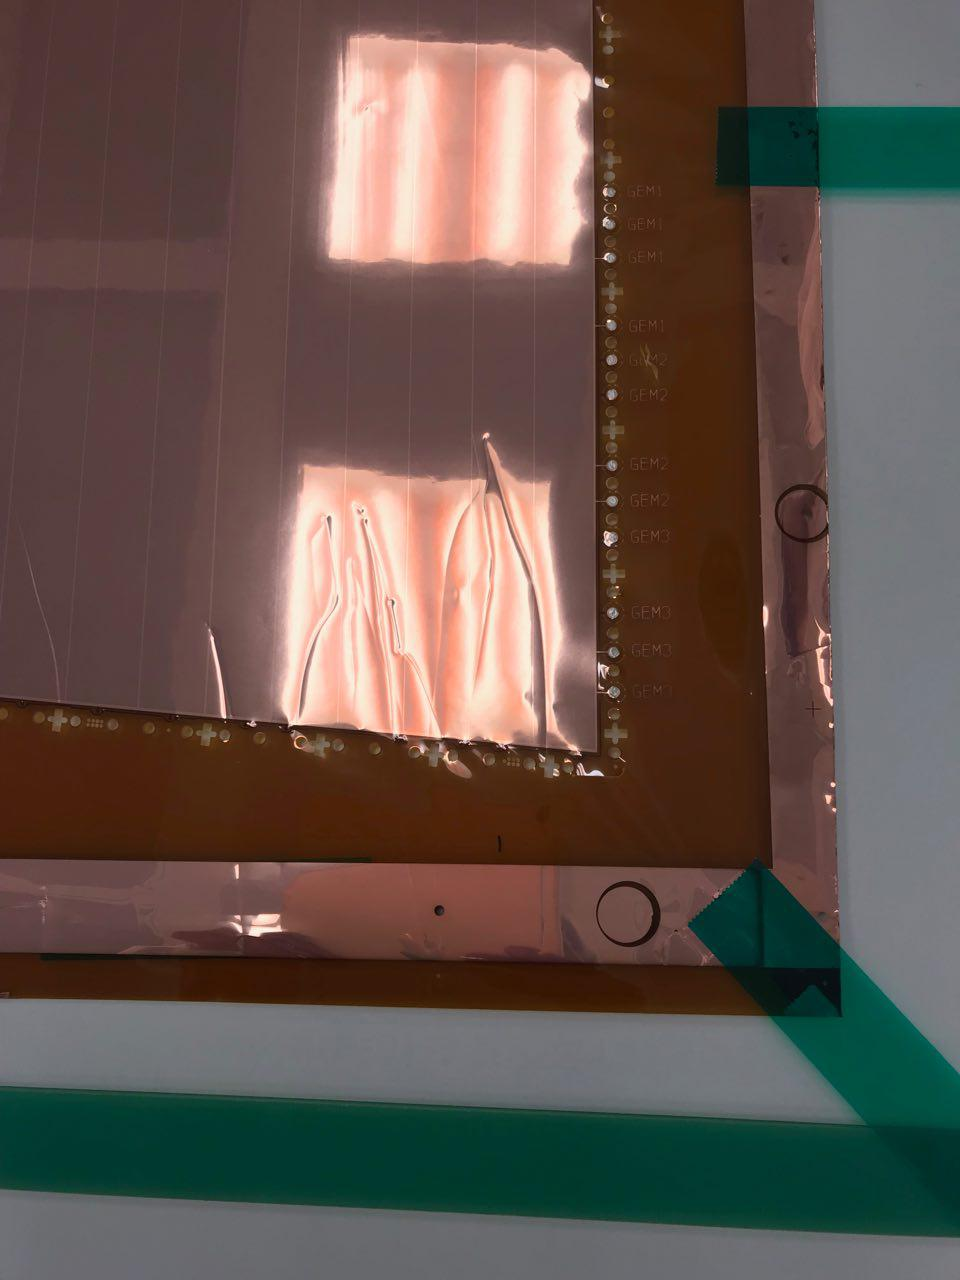
\includegraphics[width=0.40\textwidth]{damaged_case_0.jpg}
  }
  \subfloat[]{
    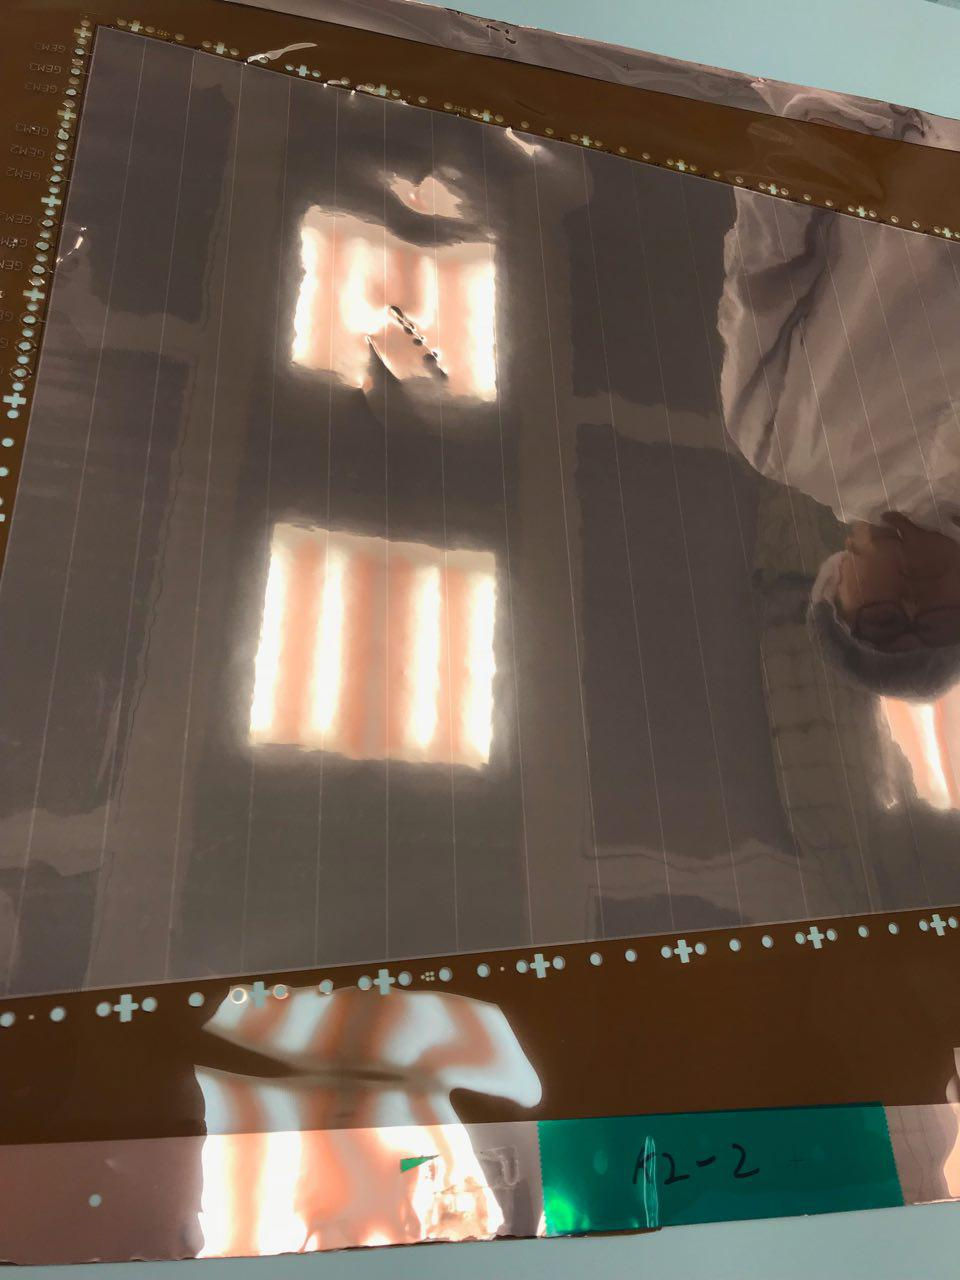
\includegraphics[width=0.40\textwidth]{damaged_case_1.jpg}
  }
  \caption[물리적 손상을 입은 포일의 예]{물리적 손상을 입은 포일의 예. 이와 같은 포일은 인수거부 할 것.}
  \label{fig:example_damaged_foils}
\end{figure}
